%
% This is the LaTeX template file for lecture notes for CS294-8,
% Computational Biology for Computer Scientists.  When preparing
% LaTeX notes for this class, please use this template.
%
% To familiarize yourself with this template, the body contains
% some examples of its use.  Look them over.  Then you can
% run LaTeX on this file.  After you have LaTeXed this file then
% you can look over the result either by printing it out with
% dvips or using xdvi.
%
% This template is based on the template for Prof. Sinclair's CS 270.

\documentclass[twoside]{article}

\usepackage{graphics}
\usepackage{amssymb}
\usepackage{tikz-cd}
\usepackage{tikz}
\usepackage{float}
\usepackage{amsmath}

\usetikzlibrary{backgrounds}
\setlength{\oddsidemargin}{0.25 in}
\setlength{\evensidemargin}{-0.25 in}
\setlength{\topmargin}{-0.6 in}
\setlength{\textwidth}{6.5 in}
\setlength{\textheight}{8.5 in}
\setlength{\headsep}{0.75 in}
\setlength{\parindent}{0 in}
\setlength{\parskip}{0.1 in}

%
% The following commands set up the lecnum (lecture number)
% counter and make various numbering schemes work relative
% to the lecture number.
%
\newcounter{lecnum}
\renewcommand{\thepage}{\thelecnum-\arabic{page}}
\renewcommand{\thesection}{\thelecnum.\arabic{section}}
\renewcommand{\theequation}{\thelecnum.\arabic{equation}}
\renewcommand{\thefigure}{\thelecnum.\arabic{figure}}
\renewcommand{\thetable}{\thelecnum.\arabic{table}}
\newcommand\equaldefine{\stackrel{\mathclap{\normalfont\mbox{def}}}{=}}
\newcommand {\cat }{%
   \mathbf%
}
\newcommand {\domain }[1] {%
  \mathrm{dom}(#1)%
}
\newcommand {\codomain }[1] {%
  \mathrm{cod}(#1)%
}
\newcommand {\idarrow}[1][] {%
  \mathbf{1} {#1}%
}


%
% The following macro is used to generate the header.
%
\newcommand{\lecture}[4]{
   \pagestyle{myheadings}
   \thispagestyle{plain}
   \newpage
   \setcounter{lecnum}{#1}
   \setcounter{page}{1}
   \noindent
   \begin{center}
   \framebox{
      \vbox{\vspace{2mm}
    \hbox to 6.28in { {\bf Topos
                        \hfill Spring 2016 } }
       \vspace{4mm}
       \hbox to 6.28in { {\Large \hfill Lecture #1: #2  \hfill} }
       \vspace{2mm}
       \hbox to 6.28in { {\it Lecturer: #3 \hfill } }
      \vspace{2mm}}
   }
   \end{center}
   \markboth{Lecture #1: #2}{Lecture #1: #2}
}

\newcommand{\fig}[3]{
			\vspace{#2}
			\begin{center}
			Figure \thelecnum.#1:~#3
			\end{center}
}
\newtheorem{ex}{Example}[section]
\newtheorem{theorem}{Theorem}[lecnum]
\newtheorem{lemma}[theorem]{Lemma}
\newtheorem{proposition}[theorem]{Proposition}
\newtheorem{claim}[theorem]{Claim}
\newtheorem{corollary}[theorem]{Corollary}
\newtheorem{definition}[theorem]{Definition}
\newenvironment{proof}{{\bf Proof:}}{\hfill\rule{2mm}{2mm}}

\newcommand{\Hom}{\mathrm{Hom}}
\newcommand{\PSh}{\mathrm{PSh}}
\newcommand{\op}{\mathrm{op}}
\newcommand{\Set}{\mathbf{Set}}

\begin{document}
\lecture{3}{13 October}{David Spivak}
\\
\section{Yoneda Embedding}

For a locally small category, a presheaf is a functor from
$C^\op \rightarrow \Set $.
The category of presheaves on $C$ is a
category whose objects are functors
$C^\op \rightarrow \Set $
and whose morphisms are natural transformations between these functors:
$$\PSh(C):=[C^\op,\Set]$$

The Yoneda embedding of $C$ is a functor from $C$ to the category of presheaves
$$Y: C \rightarrow \PSh(C) $$
which sends an object $d$ to the contravariant functor $\Hom(-, d)$:
$$ Y(d)(c) = \Hom(c,d). $$

The Yoneda lemma gives an isomorphism between the sections of a presheaf $F$ at an object $d$ and the natural transformations from the Yoneda embedding of $d$ to $F$:
$$ F(d) \cong \Hom_{\PSh(C)}(Y(d),F)$$

\section{Representable Functors}

A functor
$$ F : C^{op} \rightarrow \mathbf{Set} $$
is a representable functor if it is naturally isomorphic to $\Hom_{C}(d,-)$ from some $d \in C$,
$$ F \cong \Hom_{C}(d,-).$$

%% http://mysite.science.uottawa.ca/phofstra/MAT5147/presheaves.pdf

It follows from the definition that a presheaf is representable if it
can be expressed as something in the image of the Yoneda embedding.

For the following topos, let's determine how many representables are
each topos.

\begin{ex}
Let's consider the representables of a presheaf of the category $\star$, which has a single object and only the identity morphism.
$$\PSh(\star)  \equiv \mathbf{Set}$$
\end{ex}


The above equivalence can be observed by considering an arbitrary set $B$
and the set of mappings from $\star$.

%There seems to be some conflation of the one-object category, the one-element set here, and the object of the one-element category here.
$$\Hom(\star,B) \cong B $$

For this category, the only representable is $Y(\star)$.
$$Y(\star) = \Hom(-,\star)$$
As the category only has one element $\star$.
$$ = H (\star,\star) $$
The maps in this set is just the identity.
$$ = \{ id_{\star } \} $$
Thus it is just a point.\\

\begin{figure}[!h]
  \centering
\begin{tikzpicture}
  \draw [rounded corners=15pt] (0,0) rectangle (2,2);

  \filldraw [black] (1,1) circle (2pt);
  \node at (1.5,1.5) {$id_{\star}$};
\end{tikzpicture}\\
\end{figure}

\begin{ex}
Let's consider the representables of a two point $A,B$ category:
$$\PSh(A \cdot \: \cdot B ) \equiv \mathbf{Set} \times \mathbf{Set} $$
\end{ex}
The representables are given by
$$Y(A)=\Hom(-,A)=\Hom(A,A)=id_{A}$$
$$Y(B)=\Hom(-,B)=\Hom(B,B)=id_{B}$$
Thus the representables are just two points.\\

\begin{figure}[!h]
  \centering
\begin{tikzpicture}
  \draw [rounded corners=8pt] (0,0) rectangle (2,2);

  \filldraw [black] (1,1) circle (2pt);
  \node at (1.5,1.5) {$id_{A}$};

  \draw [rounded corners=8pt] (3,0) rectangle (5,2);

  \filldraw [black] (4,1) circle (2pt);
  \node at (3.5,1.5) {$id_{B}$};

\end{tikzpicture}\\
\end{figure}

\begin{ex}
Building on the previous example by adding $f : A \rightarrow B$ lets
consider the representables of the "function" category.
$Psh(A \cdot A  \rightarrow \cdot B )   \equiv \mbox{"functions"}$\\
\end{ex}
The representables are given by $Y(A)$,$Y(B)$.
$$Y(A)=Hom(-,A)=Hom(\{A,B,f\},A)=\{id_{A},\{\},id_{A} \rightarrow \{\} \}$$
$$Y(B)=Hom(-,B)=Hom(\{A,B,f\},B)=\{f,\{\},id_{B},f \rightarrow id_{B} \}$$
The second representable has:

\begin{figure}[!h]
  \centering
\begin{tikzpicture}
  \draw [rounded corners=8pt] (0,0) rectangle (4,2);

  \filldraw [black] (1,1) circle (2pt);
  \filldraw [gray] (3,1) circle (2pt);
  \node at (1.5,1.5) {$id_{A}$};
  \node at (2.5,1.5) {$\{\}$};


  \draw [rounded corners=8pt] (6,0) rectangle (10,2);

  \filldraw [black] (7,1) circle (2pt);
  \filldraw [black] (9,1) circle (2pt);
  \node (1) at (7,1) {};
  \node (2) at (9,1) {};
  \node at (7.5,1.5) {$f$};
  \node at (8.5,1.5) {$id_{B}$};

  \draw [->] (1) -- (2);
\end{tikzpicture}
\end{figure}

\begin{ex}
Lets consider the representatives for a category with two parallel arrows
between sets A and B.
$$Psh(A \cdot A  \rightrightarrows \cdot B ) \equiv \mbox{"graphs"}$$\\
\end{ex}
Lets can treat this category as a (multi)graphs (with loops) using the
following approach.  Lets consider the sets $A,B$ to be $V,E$ representing
vertices and edges.  Without loss of generality lets consider one of
the arrows to be the source and another to be the target.\\
\begin{figure}[H]
       \centering
\begin{tikzcd}
  V \arrow[bend left=50]{r}[name=U,above]{s}
  \arrow[bend right=50]{r}[name=D,below]{t} &
  E
\end{tikzcd}
\end{figure}
The representables are given by $Y(V)$,$Y(E)$. Lets consider the first.
$$Y(V)=Hom(-,V)=Hom(V,V)=I_{V}$$
Which is just a single point.  For the second representables there are
two hom sets to consider.
$$Y(E)=Hom(-,E)=\{s,t,I_{E}\}$$
The representables are given below.

\begin{figure}[!h]
  \centering
\begin{tikzpicture}
  \draw [rounded corners=8pt] (0,0) rectangle (2,2);

  \filldraw [black] (1,1) circle (2pt);
  \node at (1.5,1.5) {$id_{V}$};

  \draw [rounded corners=8pt] (4,0) rectangle (8,2);

  \filldraw [black] (5,1) circle (2pt);
  \filldraw [black] (7,1) circle (2pt);
  \node (1) at (5,1) {};
  \node (2) at (7,1) {};
  \node at (5,1.5) {$s$};
  \node at (7,1.5) {$t$};

  \draw [->] (1) -- node[above] {$I_{E}$} ++ (2);
\end{tikzpicture}
\end{figure}

\section{Exponential}

If $C$ is a category with products define a inner hom $f : C \times C \rightarrow C$ to
be :
$$ \forall c,d \in C : d^{c} \in C $$
an object such that there is a natural isomorphism.
$$ Hom_{C}(x,d^{c}) \cong Hom_{C}(x \cdot c,d) $$
This inner hom $f$ is defined as the exponential and is always defined for topoi.

Given presheaves $F,G : C^{op} \rightarrow \mathbf{Set} $ let consider what is:

$$F^{G} : C^{op} \rightarrow \mathbf{Set} $$

By looking at representables :

$$Hom_{Psh(c)}(Y(c),F^{G}) = Hom(Y(c) \times G,F)$$

\begin{ex}
  Consider two sets $F,G$\\
\begin{figure}[!h]
  \centering
\begin{tikzpicture}
  \draw [rounded corners=8pt] (0,0) rectangle (4,2);

  \filldraw [black] (1,1) circle (2pt);
  \filldraw [black] (2,1) circle (2pt);
  \filldraw [black] (3,1) circle (2pt);
  \node at (1.5,1.5) {$F$};

  \draw [rounded corners=8pt] (6,0) rectangle (10,2);

  \filldraw [black] (7,1) circle (2pt);
  \filldraw [black] (8,1) circle (2pt);
  \node at (7.5,1.5) {$G$};

  \node (1) at (4.2,1) {};
  \node (2) at (5.8,1) {};

  \draw [<-] (1) -- node[above] {$F^{G}$} ++ (2) ;
\end{tikzpicture}
\end{figure}

  What is $F^{G}:\star^{op} \rightarrow \mathbf{Set}$\\
\end{ex}
  Consider:
  $$F^{G} = Hom(Y(c) \times G,F)$$
  As we are considering the one point set.
  $$= Hom(G,F)$$
  Using the cardinality of the sets provided $G=2$ and $F=3$
  $$= 2^3$$

\begin{ex}
  Consider two sets $F,G$\\
\begin{figure}[!h]
  \centering
\begin{tikzpicture}
  \draw [rounded corners=8pt] (0,0) rectangle (5,2);

  \draw [rounded corners=8pt] (0.2,0.5) rectangle (1.8,1.5);

  \filldraw [black] (0.5,1) circle (2pt);
  \filldraw [black] (1.3,1) circle (2pt);
  \node at (1.5,1.3) {$A$};

  \draw [rounded corners=8pt] (2.0,0.5) rectangle (4.8,1.5);

  \filldraw [black] (2.6,1) circle (2pt);
  \filldraw [black] (3.4,1) circle (2pt);
  \filldraw [black] (4.2,1) circle (2pt);
  \node at (4.0,1.3) {$B$};

  \node at (4.0,1.8) {$F$};


  \draw [rounded corners=8pt] (8,0) rectangle (12,2);

  \draw [rounded corners=8pt] (8.2,0.5) rectangle (9.8,1.5);

  \filldraw [black] (8.5,1) circle (2pt);
  \filldraw [black] (9.3,1) circle (2pt);
  \node at (9.5,1.3) {$A$};

  \draw [rounded corners=8pt] (10.2,0.5) rectangle (11.8,1.5);
  \node at (8.8,1.8) {$G$};
  \node at (10.5,1.3) {$B$};


  \node (1) at (5.2,1) {};
  \node (2) at (7.8,1) {};

  \draw [<-] (1) -- node[above] {$F^{G}$} ++ (2) ;
\end{tikzpicture}
\end{figure}

  What is $F^{G}: \{ A,B \} \rightarrow \mathbf{Set}$\\
\end{ex}

$$F^G(A) = Hom (Y(A) \times G , F) = 2^2$$
$$F^G(B) = Hom (Y(B) \times G , F) = 3^0$$

\section{Mighty Morphing functions}
\subsection{Monomorphism}
Let $f : X \rightarrow Y$ be a function, $f$ is a monomorophism (or monic) if for any set $A$ and
pairs of functions $g , g' : A \rightarrow X$ the $f \circ g = f \circ g' \Rightarrow g = g'$.

\begin{figure}[H]
       \centering
\begin{tikzcd}
  A   \arrow[bend left=50]{r}[name=U,above]{g}
      \arrow[bend right=50]{r}[name=D,below]{g'} &
  X   \arrow[]{r}[name=D]{f} &
  Y
\end{tikzcd}
\end{figure}

\begin{claim}
  $f$ is a monomorphism iff it is injective.
\end{claim}
\begin{proof}
  Assume $f$ is a monomorphism.  Show that it is injective, that is for any $\forall x,y \in X : x \neq y$
  implies $f(x) \neq f(y)$.  Consider the case if $f$ is not injective with  $x \neq y$
  and  $f(x) = f(y)$ consider $A = \{ \star \}$
  and define two functions $g( \star ) = x$ and $g'( \star ) = y$.  It follows from the definition that
  $f \circ g(\star) = f \circ g'(\star)$ contradicting the momorophism condition that
  $g' = g$.\\

  Assume $f$ is injective lets show $f$ is a monomorphism.  Consider an arbitrary $A$ and $g, g' : A \rightarrow X$
  and $g \neq g'$ such that $f \circ g = f \circ g'$.  Consider the contradiction where  $g \neq g'$ and the functions
  differ on point $g(\star) = g'(\star)$.  As $f$ is injective then $f \circ g(\star) = f \circ g'(\star) $ contradicting
  $f \circ g \neq f \circ g'$.

 \end{proof}

\begin{claim}
  if $f : X \rightarrow Y , g : Y \rightarrow Z$ are monomorphisms and composable then $f \circ g : X \rightarrow Z $ is an monorphisms.
\end{claim}


\begin{proof}
  This follows from the definition of monomorphisms, consider $x_1, x_2 \in X$ such that $f \circ g (x_1) = f \circ g (x_2)$ as
  $f$ is injective $g(x_1) = g(x_2)$ and $g$ is injective thus $x_1 = x_2$.
\end{proof}

\subsection{Epimorphism}

Let $f : A \rightarrow Y$, $f$ be a function, $f$ is an epimorphism (or epic), if for all
sets $B$ and functions $h,h' : Y \rightarrow B$ then $h \circ f = h' \circ f \Rightarrow h = h' $.

\begin{figure}[H]
       \centering
\begin{tikzcd}
  X   \arrow[]{r}[name=D]{f} &
  Y   \arrow[bend left=50]{r}[name=U,above]{h}
      \arrow[bend right=50]{r}[name=D,below]{h'} &
  B
\end{tikzcd}
\end{figure}

\begin{claim}
  $f$ is a epimorphism iff it is surjective.
\end{claim}

\begin{proof}
  Assume $f$ is an an epimorphism show $f$ is surjective.  Assume $f$ was
  not surjective then $\exists y \in Y$ and $y \notin f(x)$ consider $B = \{ 0,1 \}$.
  Define :
  $$h(y)=1$$
  $$h'(y)=
  \begin{cases}
    0, & y \in f(X) \\
    1, & y \notin f(X) \\
  \end{cases}$$
  $h \circ f = h' \circ f$ by the definition of epimorphism $h = h'$ which contradicts
  the definitions of $h,h'$.\\

  Assume $f$ is surjective show $f$ is an epimorphism.  Assume $h \circ f = h' \circ f$
  yet $h \neq h'$ consider a point in $\star \in Y$ where these two functions differ
  $h(\star) \neq h'(\star)$ as $f$ is surjective consider an $x \in X : f(x) = \star$
  then $h \circ f(x) \neq h' \circ f(x)$ leading to a contradiction.
\end{proof}


\footnote{ Reference : \cite[Chapter~1.2]{popescu2012theory} \cite[p.~104]{spivak2014category} }

\section{Subobject}

A subobject of an object $X \in C$ is a monomorphism $m$

$$ m : M \rightarrow  X$$

A subobject defines a subset of $X$ namely the image of $m$.

$$ m(M) \subset X $$

A category of subjects $Sub_{C}(X)$ is be defined with objects
being monics. A morphism $f$ is defined between monics $m,m'$.

\begin{figure}[H]
       \centering
\begin{tikzcd}
  M  \arrow[]{r}[name=U,above]{f}
     \arrow[]{dr}[name=U,left]{m} & M' \arrow[]{d}[name=U,right]{m'} \\
                                   & X \\
\end{tikzcd}
\end{figure}

\footnote{ Reference : \cite[Chapter~5]{awodey2006category} }

\section{Pullback}

Consider two morphisms $f : X \rightarrow Z $ and $g :  Y \rightarrow Z$

\begin{figure}[H]
       \centering
\begin{tikzcd}
                                 & Y \arrow[]{d}[name=U,right]{g} \\
  X \arrow[]{r}[name=U,below]{f} & Z \\
\end{tikzcd}
\end{figure}

The fiber product is defined as :

$$ X \times_{Z} Y = \{ (x,z,y) | f(x) = z = g(y) \} $$

Projections from the fiber product can be defined as

$$ \pi_{1} : X \times_{Z} Y  \rightarrow X $$
$$ \pi_{2} : X \times_{Z} Y  \rightarrow Y $$

The following diagram commutes.

\begin{figure}[H]
       \centering
\begin{tikzcd}
  X \times_{Z} Y \arrow[]{d}[name=U,left]{\pi_{1}}
                 \arrow[]{r}[name=U,above]{\pi_{2}} & Y \arrow[]{d}[name=U,right]{g} \\
  X \arrow[]{r}[name=U,below]{f} & Z \\
\end{tikzcd}
\end{figure}

There is a universial property that states that given another
set $U$ and morphisms $s : U \rightarrow Y ,t : U \rightarrow X $
there exists a function $h : U \rightarrow X \times_{Z} Y$
such that the following diagram commutes.


\begin{figure}[H]
 \centering
 \begin{tikzcd}
   U \arrow[]{dr}[name=U,right=10]{h}
     \arrow[bend left=30]{drr}[name=U,right=10]{s}
     \arrow[bend right=30]{ddr}[name=U,left=10]{t}
   &                &   \\
   & X \times_{Z} Y \arrow[]{d}[name=U,left]{\pi_{1}}
                 \arrow[]{r}[name=U,above]{\pi_{2}} & Y \arrow[]{d}[name=U,right]{g} \\
   & X \arrow[]{r}[name=U,below]{f} & Z \\
\end{tikzcd}
\end{figure}

\section{Subobject classifier}

The subset relation $A \subset B$ can be
charaterized in two manners.

The first is by a monic $m : A \rightarrow B$ which is
an inclusion.

The second is by the characteristic function

$$\phi_A(x) =
  \begin{cases}
    0, & x \in S \\
    1, & x \notin S \\
  \end{cases}$$

Lets consider the domain of $\phi_A = \{0,1\}$.  The function
$true$ is defined as

$$true : \{ 0 \} \rightarrow \{ 0, 1 \} $$

This gives the following diagram

\begin{figure}[H]
       \centering
\begin{tikzcd}
  A \arrow[]{r}[name=U,above]{a}
    \arrow[]{d}[name=U,left]{m}         & \{ 0 \}    \arrow[]{d}[name=U,right]{true} \\
  B \arrow[]{r}[name=U,above]{\phi_{A}} & \{ 0, 1 \}  \\
\end{tikzcd}
\end{figure}

$a : A \rightarrow \{ 0 \} $ is the unique function from $S$
to the terminal object $\{ 0 \}$, such that the diagram is a pullback.


\begin{definition}
For any category $C$ a subobject classifier is a monomorphism
$$true : T \rightarrow \Omega $$
Such that for any monomorphism $m \in C$ :
$$ m : A \rightarrow B $$
There exists an unique arrow $\phi$ (the characteristic function)
$$\phi : B \rightarrow \Omega $$
Such that there is pull back diagram.\\

\begin{figure}[H]
       \centering
\begin{tikzcd}
  A \arrow[d]{}[name=m,left]{m} \arrow[r] & T \arrow[d]{}[name=t,right]{true}  \\
  B \arrow[r]{}[name=phi,below]{\phi} & \Omega \\
\end{tikzcd}
\end{figure}
\end{definition}


\bibliographystyle{plain}
\bibliography{notes}

\end{document}
